\documentclass[a4paper,11pt]{report}
\usepackage{color}
\usepackage{graphicx}
\usepackage{subcaption}
\usepackage{amsmath}
\usepackage{tikz}
\usepackage{listings}
\definecolor{codegreen}{rgb}{0,0.6,0}
\definecolor{codegray}{rgb}{0.5,0.5,0.5}
\definecolor{codepurple}{rgb}{0.58,0,0.82}
\definecolor{backcolour}{rgb}{0.95,0.95,0.92}
 
\lstdefinestyle{mystyle}{
    backgroundcolor=\color{backcolour},   
    commentstyle=\color{codegreen},
    keywordstyle=\color{magenta},
    numberstyle=\tiny\color{codegray},
    stringstyle=\color{codepurple},
    basicstyle=\footnotesize,
    breakatwhitespace=false,         
    breaklines=true,                 
    captionpos=b,                    
    keepspaces=true,                 
    numbers=left,                    
    numbersep=5pt,                  
    showspaces=false,                
    showstringspaces=false,
    showtabs=false,                  
    tabsize=2
}
 
\lstset{style=mystyle}
\usetikzlibrary{automata,positioning}
\graphicspath{ {images/} }
\begin{document}
\title{\color{red}CARNEGIE MELLON UNIVERSITY\\
APPLIED STOCHASTIC PROCESSES  (COURSE 18-751)\\
HOMEWORK 1}
\author{Daniel Marew}
\date{\today}
\maketitle
\newpage
\section*{Q.1 prove with Venn diagrams}
\subsection*{(a) $A \cap B^c = A-B$}
\begin{figure}[h]
    \centering
    \begin{subfigure}[b]{0.25\textwidth}
        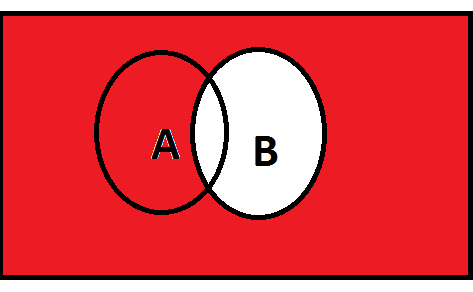
\includegraphics[width=\textwidth]{BC}
        \caption{$B^c$}
    \end{subfigure}
 ~
    \begin{subfigure}[b]{0.25\textwidth}
        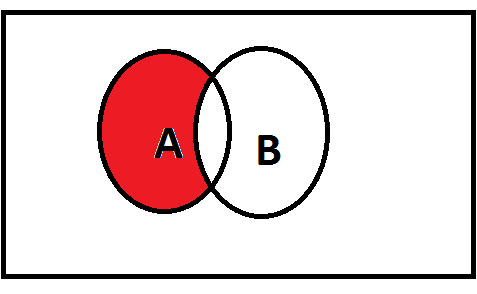
\includegraphics[width=\textwidth]{AnBc}
        \caption{$A \cap B^c$}
    \end{subfigure}
 ~
    \begin{subfigure}[b]{0.25\textwidth}
        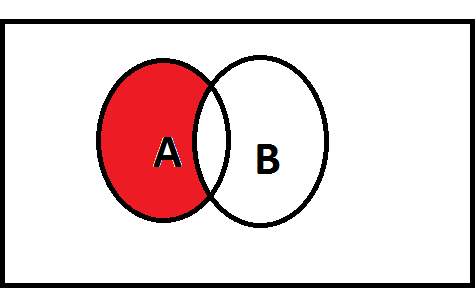
\includegraphics[width=\textwidth]{A-B}
        \caption{$A-B$}
        \label{fig:mouse}
    \end{subfigure}
    \caption{}

\end{figure}
this implies $A \cap B^c = A-B$ is true
\subsection*{(b) $A \cup B^c = (A^c\cap B)^c$}
\begin{figure}[hb]
  \centering
    \begin{subfigure}[b]{0.25\textwidth}
        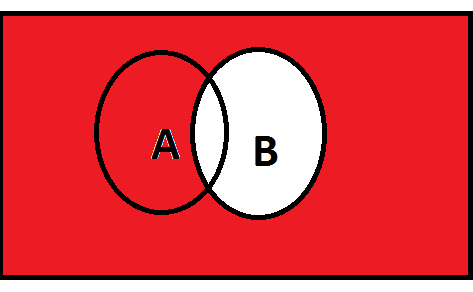
\includegraphics[width=\textwidth]{BC}
        \caption{$B^c$}
    \end{subfigure}
 ~
    \begin{subfigure}[b]{0.25\textwidth}
        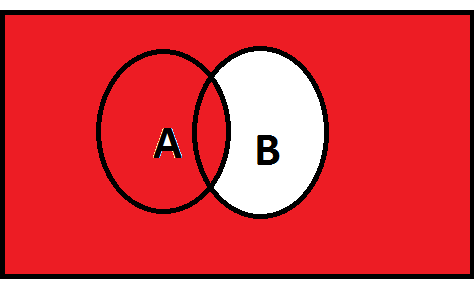
\includegraphics[width=\textwidth]{AuBc}
        \caption{$A \cup B^c$}
    \end{subfigure}
 ~
    \begin{subfigure}[b]{0.25\textwidth}
        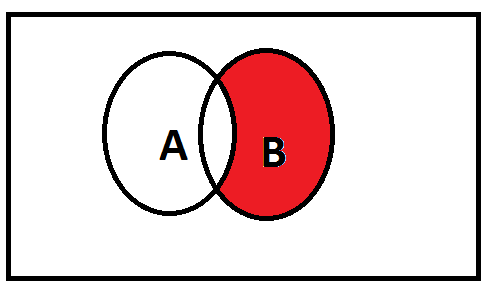
\includegraphics[width=\textwidth]{AcnB}
        \caption{$A^c\cap B$}
        \label{fig:mouse}
    \end{subfigure}
 ~
    \begin{subfigure}[b]{0.25\textwidth}
        \includegraphics[width=\textwidth]{AcnBc}
        \caption{$(A^c \cap B)^c$}
        \label{fig:mouse}
    \end{subfigure}
    \caption{}
\end{figure}
hence $A \cup B^c = (A^c\cap B)^c$ is true
\subsection*{(c) $B-A \neq A-B$}
\begin{figure}[h]
    \centering
    \begin{subfigure}[b]{0.25\textwidth}
        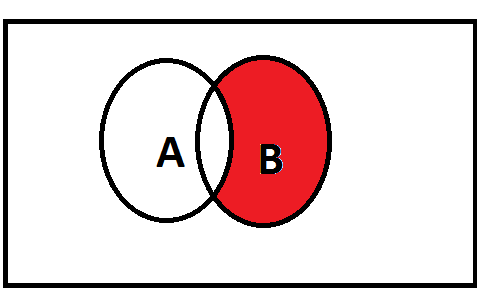
\includegraphics[width=\textwidth]{B-A}
        \caption{$B-A$}
    \end{subfigure}
    \begin{subfigure}[b]{0.25\textwidth}
        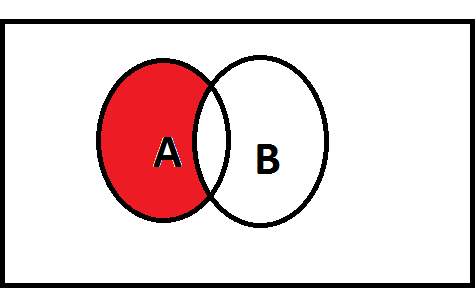
\includegraphics[width=\textwidth]{A-B}
        \caption{$ A-B$}
    \end{subfigure}
    \caption{}
\end{figure}
therefor $B-A \neq A-B$ is true
\newpage
\section*{Q.2}
\begin{figure}[h]
 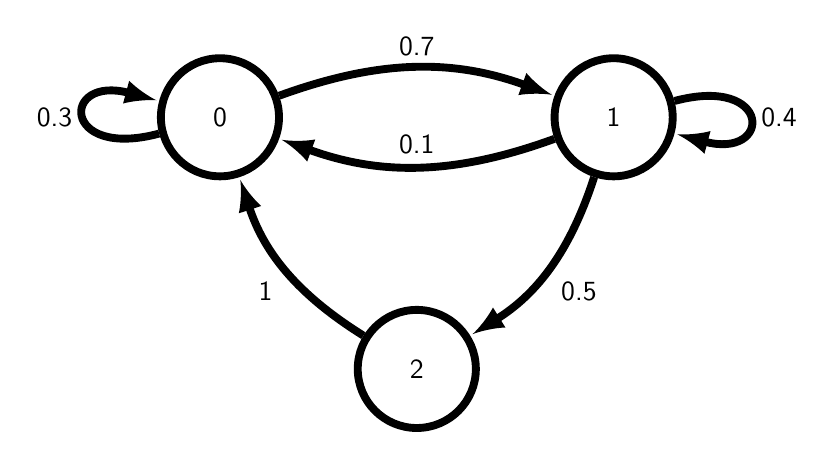
\begin{tikzpicture}[font=\sffamily]
        % Setup the style for the states
        \tikzset{node style/.style={state, 
                                    minimum width=1.5cm,
                                    line width=1mm,
                                   }}
        % Draw the states
        \node[node style] at (0, 0)     (bull)     {0};
        \node[node style] at (5, 0)     (bear)     {1};
        \node[node style] at (2.5, -3.196) (stagnant) {2};
 
        % Connect the states with arrows
        \draw[every loop,
              auto=right,
              line width=1mm,
              >=latex]
            (bull)     edge[bend left=20, auto=left] node {0.7} (bear)
            (bear)     edge[bend left=20]            node {0.1} (bull)
            (bear)     edge[bend left=20, auto=left] node {0.5} (stagnant)
            (stagnant) edge[bend left=20, auto=left] node {1} (bull)
            (bull) edge[loop left] node {0.3} (bull)
	 (bear) edge[loop right] node {0.4} (bear);
            
    \end{tikzpicture}
    \caption{MC}
     \label{fig:MC1}
\end{figure}

\subsection*{(a) Irreduciblity and periodicity }
\subsubsection*{Irreduciblity}
	
A markov chain is said to be Irreducible if
\begin{equation}
\forall i,j \in S, \exists m < \infty : P(X_{n+m} = j|X_n=i )>0
\end{equation}•
i.e regardless the present state we can reach any other state in finit time.\cite{irreducible}
On the Markov Chain in figure \ref{fig:MC1} we can go from any of the  states  to the other states in a finit number of steps hence it is irreducible.
\subsubsection*{Periodicity}
for an irreducible Markov Chain the periodicity of state $i$ is defined by
\begin{equation}
d(i)= g.c.d\{n\geq 1 | P^n(i,i)>0\}
\end{equation}•\\
and $d(i)$ has the same value $d$ for all $i$. A Markov Chain is said to be aperiodic if $d=1$ \cite{text}\\\\
for the Markov Chain on figure \ref{fig:MC1} at $n = 1$
$$
P^1=\begin{bmatrix} 
0.3 & 0.7 & 0 \\
0.1 & 0.4 & 0.5\\
1    & 0     &0
\end{bmatrix}
$$
already we can find $ i$ such that $P(i,i)>0$ . For example $P(0,0)=0.3>0$ and the $ g.c.d $ of any set of integers that contains $1$ is $1$.
hence figure \ref{fig:MC1} is aperiodic.\\\\
Ans.
\textbf{Irreducible} and \textbf{Aperiodic}. 

\subsection*{(b) invariant distribution ($\pi$) }

\begin{eqnarray}
\pi_j = \sum_{k=1}^{n} \pi_k p_{kj}
\end{eqnarray}•

\begin{eqnarray}
\pi_0 = \pi_0 P_{00} + \pi_1 P_{10} + \pi_2 P_{20}\\
\pi_1 = \pi_0 P_{01} + \pi_1 P_{11} + \pi_2 P_{21}\\
\pi_2 = \pi_0 P_{02} + \pi_1 P_{12} + \pi_2 P_{22}
\end{eqnarray}

i.e $\pi = \pi P$\\

$$
P=\begin{bmatrix} 
0.3 & 0.7 & 0 \\
0.1 & 0.4 & 0.5\\
1    & 0     &0
\end{bmatrix}
$$


\begin{eqnarray}
\pi_0 = 0.3\pi_0+ 0.1\pi_1 + \pi_2 \\
\pi_1 = 0.7\pi_0+ 0.4\pi_1  \\
\pi_2 = 0.5\pi_1\\ 
\pi_0+\pi_1+\pi_2 = 1
\end{eqnarray}•

lets write everything interms of $\pi_1$\\
\begin{eqnarray}
\pi_1=\pi_1\\
\pi_2=0.5\pi_1\\
\pi_0 = 0.3\pi_0+0.1\pi_1+0.5\pi_1\\
0.7\pi_0=0.6\pi_1\\
\pi_0 = \frac{6}{7}\pi_1\\
\pi_0+\pi_1+\pi_2=\frac{6}{7}\pi_1+\pi_1+0.5\pi_1=1
\end{eqnarray}•
\begin{eqnarray}
\frac{33}{14}\pi_1=1\\
\pi_1=\frac{14}{33}\\
\pi_0=\frac{6}{7}.\frac{14}{33}=\frac{4}{11}\\
\pi_2=0.5.\frac{14}{33}=\frac{7}{33}
\end{eqnarray}•
Ans.
$$
\pi = \begin{bmatrix}
\frac{4}{11} \quad \frac{14}{33}\quad \frac{7}{33}   
\end{bmatrix}•
$$

$$
\pi \approx \begin{bmatrix}
0.3636 \quad 0.4242 \quad   0.2121
\end{bmatrix}•
$$
\subsection*{(c) Expected Time from 0 to 2}

We can calculate $\beta(0)$ \\\\ i.e\\$\beta(0)= E[$average time to reach $2$ $|$ current state is $0] $
\begin{eqnarray}
\beta(2) = 0\\
\beta(0) = 1+0.7\beta(1) + 0.3\beta(0)\\
\beta(1) = 1+0.1\beta(1) +0.4\beta(1) + 0.5\beta(2) 
\end{eqnarray}•

since $\beta(2)=0$
\begin{eqnarray}
\beta(1) = 1+0.1\beta(0) + 0.4\beta(1)
\beta(0) = 1+0.3\beta(0) + 0.7\beta(1)
\end{eqnarray}•

\begin{equation}\label{eq:1}
0.7\beta(0)-0.7\beta(1) = 1
\end{equation}•
\begin{equation}\label{eq:2}
0.6\beta(1)-0.1\beta(0) = 1
\end{equation}•
solving the equations (\ref{eq:1}) and (\ref{eq:2}) we get $\beta(0) \approx 3.708$ and $\beta(1)\approx 2.286$\\\\
Ans.
So the expected time from $0$ to $2$ is $ 3.708$


\newpage

\subsection*{(d) Probability that starting from 0, the MC has reached 2 after $n$-steps  vs $ n$}

The $n$-step transition probability is defined by \cite{mit}\\
\begin{equation}
r_{ij}(n) = P(X_n = j | X_0 = i)
\end{equation}
$r_{ij}(n)$ is the probability that the state after n time periods will be $j$, given that the current state is $i$.\\\\
We can get $r_{ij}(n)$ by using  Chapman-Kolmogorov Equation \cite{mit}

\begin{equation}
r_{ij}(n) = \sum_{k=1}^{m}r_{ik}(n - 1)p_{kj}
\end{equation}•
for $n > 1$, and all $i$, $j$, starting with
$$r_{ij}(1) = P_{ij}$$
[CODE] = Code Appendix 2. d 
\begin{figure}[h]
\hspace*{-4cm}
        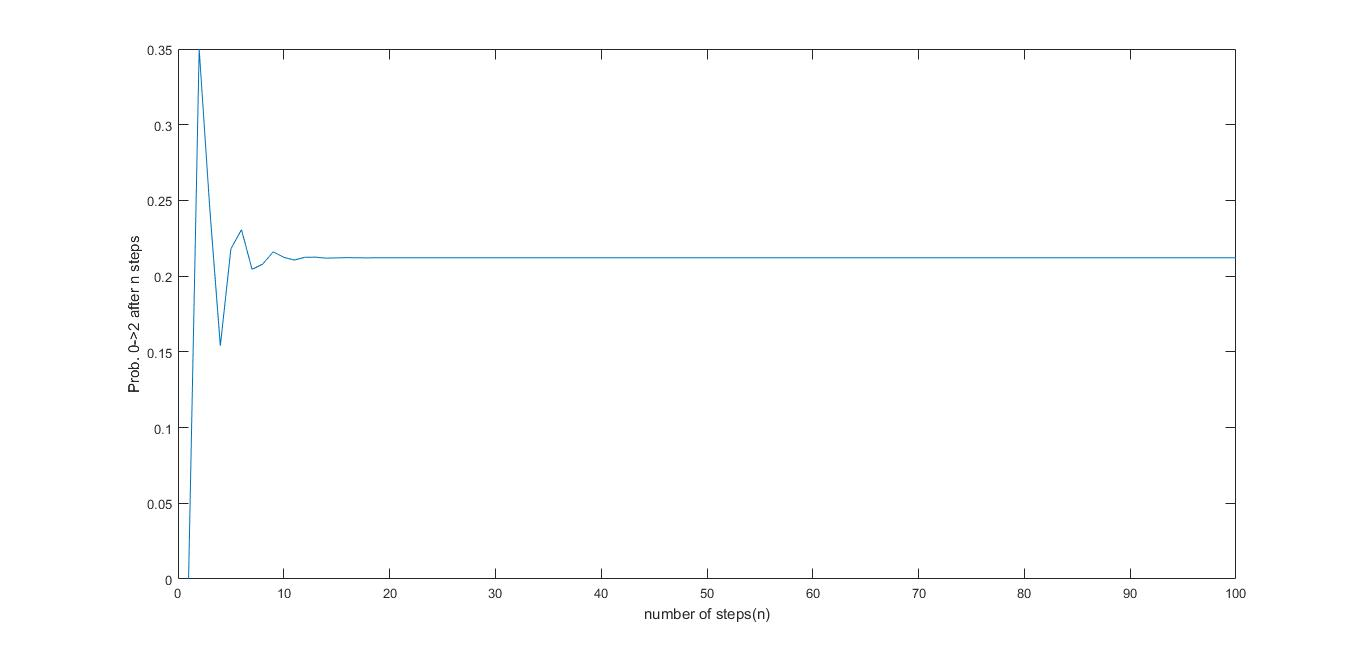
\includegraphics[scale=0.45]{2d}
        \caption{Probability that starting from 0, the MC has reached 2 after $n$-steps  vs $ n$}
\end{figure}
\newpage
\subsection*{(e) Fraction of Time}
[CODE] = Code Appendix 2. e 
\begin{figure}[h]
\hspace*{-6cm}
        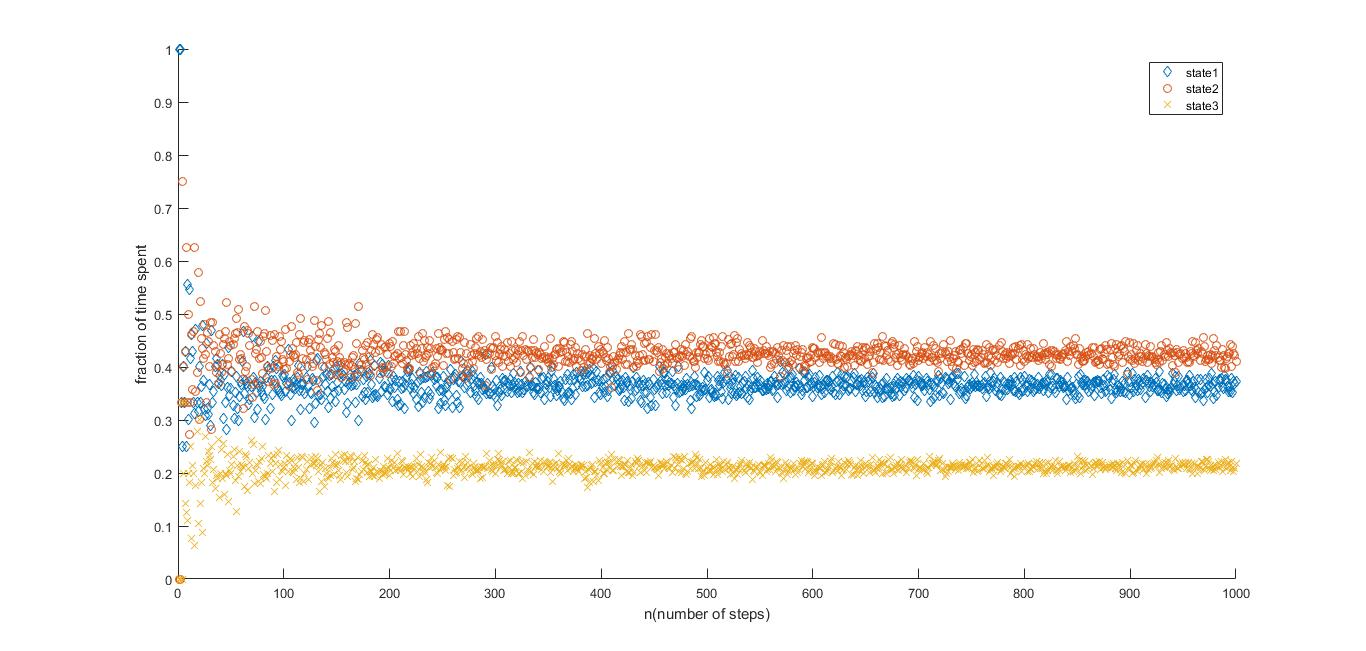
\includegraphics[scale=0.6]{2e}
        \caption{Fraction of time it spends in each of the states  vs $ n$}
\end{figure}\\
Remark:\\
On every run we get slightly different outcome just because of the inherent randomness of the Markov chain.
But for large $n$ all of the states will converge to the values in the invariant distribution.
\newpage
\subsection*{(f) $\pi_n$  vs $n$}
[CODE] = Code Appendix 2. f 
\begin{figure}[htbp]
\hspace*{-6cm}
        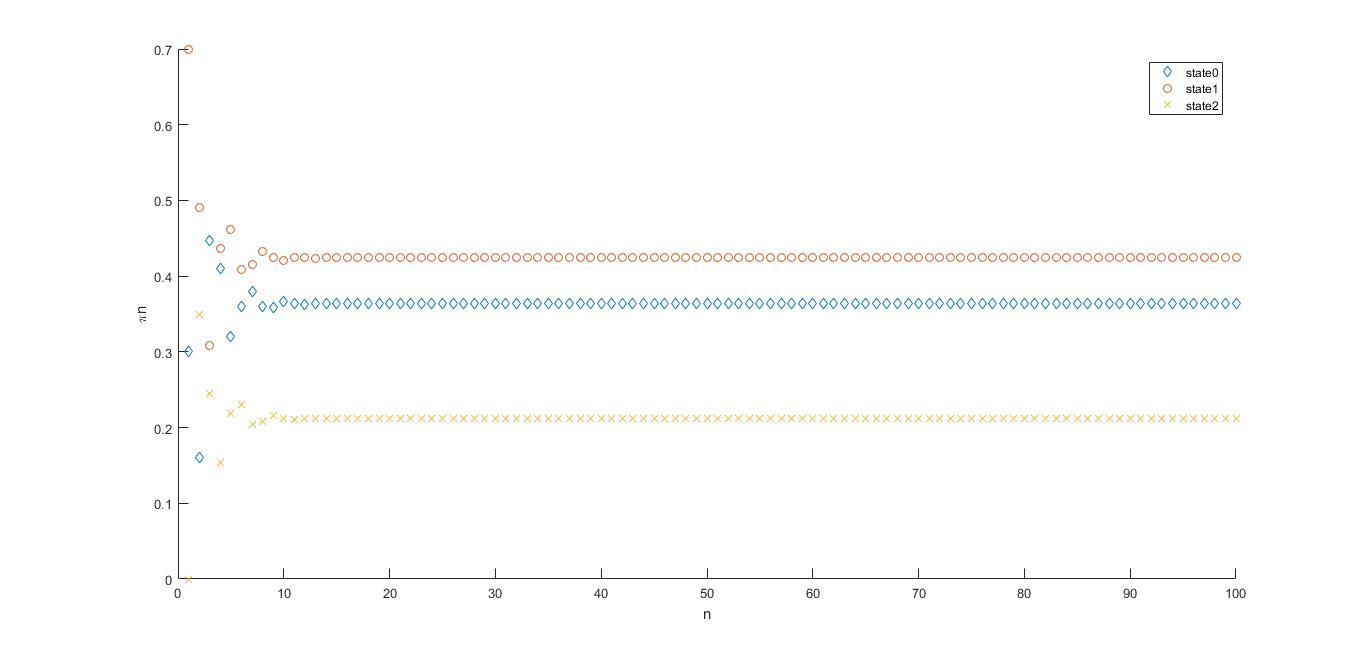
\includegraphics[scale=0.5]{2f}
        \caption{$\pi_n$ vs $n$}
\end{figure}
\newpage 
\section*{Q3}
\subsection*{(a) Page Rank}
We can rank the states by their value in the invariant distribution($\pi$)\\\\
1. state(page) 1\\
2. state(page) 0\\
3. state(page) 2\\
\subsection*{(b) Removing self connections and Normalizing}
After removing the self connections, there are an infinit number of ways of normalizing the Markov Chain. One way is \\
\begin{figure}[h]
 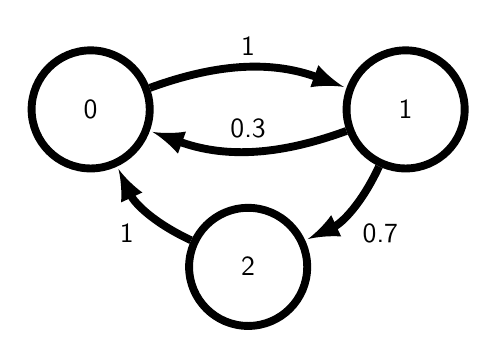
\begin{tikzpicture}[font=\sffamily]
        % Setup the style for the states
        \tikzset{node style/.style={state, 
                                    minimum width=1.5cm,
                                    line width=1mm,
                                   }}
        % Draw the states
        \node[node style] at (3, 0)     (bull)     {0};
        \node[node style] at (7, 0)     (bear)   {1};
        \node[node style] at (5, -2) (stagnant) {2};
 
        % Connect the states with arrows
        \draw[every loop,
              auto=right,
              line width=1mm,
              >=latex]
            (bull)     edge[bend left=20, auto=left] node {1} (bear)
            (bear)     edge[bend left=20]            node {0.3} (bull)
            (bear)     edge[bend left=20, auto=left] node {0.7} (stagnant)
            (stagnant) edge[bend left=20, auto=left] node {1} (bull)  ;

             
            %(bull) edge[loop left] node {0.3} (bull)
	 %(bear) edge[loop right] node {0.4} (bear);
            
    \end{tikzpicture}
    \caption{Updated MC}
\end{figure}

\subsection*{(c) Adding States to Trick the MC}
After adding 1a and 0a  we get a Markov Chain that looks like figure \ref{fig:MC3} 
\begin{figure}[h]
 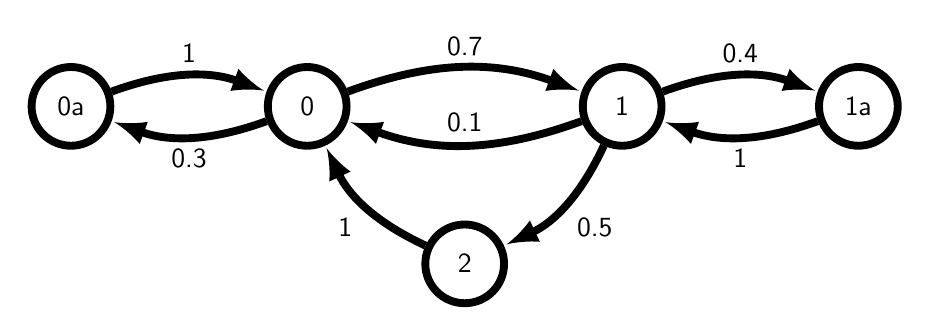
\begin{tikzpicture}[font=\sffamily]
        % Setup the style for the states
        \tikzset{node style/.style={state, 
                                    minimum width=1cm,
                                    line width=1mm,
                                   }}
        % Draw the states
        \node[node style] at (3, 0)     (bull)     {0};
        \node[node style] at (7, 0)     (bear)   {1};
        \node[node style] at (10, 0)    (d1)     {1a};
        \node[node style] at (0, 0)      (d2)     {0a};
        \node[node style] at (5, -2) (stagnant) {2};
 
        % Connect the states with arrows
        \draw[every loop,
              auto=right,
              line width=1mm,
              >=latex]
            (bull)     edge[bend left=20, auto=left] node {0.7} (bear)
            (bear)     edge[bend left=20]            node {0.1} (bull)
            (bear)     edge[bend left=20, auto=left] node {0.5} (stagnant)
            (stagnant) edge[bend left=20, auto=left] node {1} (bull)
            (d2) edge[bend left=20, auto=left] node {1} (bull)
            (bull) edge[bend left=20, auto=left] node {0.3} (d2)
            (d1) edge[bend left=20, auto=left] node {1} (bear)
            (bear) edge[bend left=20, auto=left] node {0.4} (d1)  
            ;
  
    \end{tikzpicture}
    \caption{Updated MC}
    \label{fig:MC3}
    \end{figure}
$$
P=\begin{bmatrix} 
0&1&0&0&0\\
0.3&0&0.7& 0&0 \\
0&0.1&0&0.5&0.4\\
0&1&0&0&0\\
0&0&1&0&0\\

\end{bmatrix}
$$

\begin{eqnarray}
\pi_{0a} = 0.3\pi_0 \\
\pi_0 = \pi_{0a}+ 0.1\pi_1 + \pi_2  \\
\pi_1 = 0.7\pi_0+\pi_{1a}\\ 
\pi_2 = 0.5\pi_1\\ 
\pi_{1a} = 0.4\pi_1\\ 
\pi_{0a}+\pi_0+\pi_1+\pi_2+\pi_{1a} = 1
\end{eqnarray}•

lets write everything interms of $\pi_1$\\

\begin{eqnarray}
\pi_1=\pi_1\\
\pi_2=0.5\pi_1\\
\pi_{1a}=0.4\pi_1\\
\pi_0 = 0.3\pi_0 + 0.1\pi_1 + 0.5\pi_1\\
0.7\pi_0=0.6\pi_1\\
\pi_0 = \frac{6}{7}\pi_1\\
\pi_{0a} = 0.3.\frac{6}{7}\pi_1=\frac{18}{70}\pi_1\\
\frac{18}{70}\pi_1+\frac{6}{7}\pi_1+\pi_1+\frac{1}{2}\pi_1+\frac{4}{10}\pi_1 = 1\\
\pi_1 = \frac{70}{211}\approx 0.331\\
\end{eqnarray}•
similarly  $\pi_{oa} = \frac{18}{70}\pi_1\approx0.085$, $\pi_0=\frac{6}{7}\pi_1\approx0.284$, $\pi_2=0.5\pi_1\approx0.165$, $\pi_{1a}=0.4\pi_1\approx0.132$
$$
\pi = \begin{bmatrix}
0.085 \quad 0.284 \quad 0.331 \quad 0.165 \quad 0.132    
\end{bmatrix}•
$$
\\\\\\\\\\We can rank the states(0, 1  and 2 ) by their value in the invariant distribution($\pi$) form highest to lowest\\\\
1. state(page) 1\\
2. state(page) 0\\
3. state(page) 2\\


for the MC in (b)
\begin{eqnarray}
\pi_0  = 0.3\pi_1 + \pi_2\\
\pi_1  = \pi_0\\
\pi_2  = 0.7\pi_1\\
\pi_0+\pi_1+\pi_2=1
\end{eqnarray}•
solving the above equations we get\\
$$
\pi = \begin{bmatrix}
\frac{10}{27} \quad \frac{10}{27} \quad \frac{7}{27}    
\end{bmatrix}•
$$\\
So the ranking for (b) would be \\
1. state(page) 1 = state(page) 0 \quad i.e page1 and page 2 have the same rank\\
2. state(page) 2\\\\
Remark:\\
Compared to (a) adding the new states 0a and 1a do not change the ranking. On the other hand in (b), after removing and normalizing it, Pages 0 and 1 will have the same ranking because the exit probabilty  from 0 to 1 is 1(i.e if we are at Page 0 the next Page we will look at is guaranteed to be Page 1). In all cases page 2 is ranked last.

\newpage
\begin{appendix}
\section*{Code Appendix}
\subsection*{2. d}\label{test2d}
\lstinputlisting[language=Octave]{chapmanKolmogorov.m}  
\lstinputlisting[language=Octave]{test2d.m}  
\subsection*{2. e \cite{text} Appendix C.3}\label{test2e}
\lstinputlisting[language=Octave]{discrete.m}
\lstinputlisting[language=Octave]{simMC.m}  
\newpage

\lstinputlisting[language=Octave]{get_frac_dist.m}  

\lstinputlisting[language=Octave]{test2e.m} 
\newpage
\subsection*{2. f}
\lstinputlisting[language=Octave]{PI.m}
\lstinputlisting[language=Octave]{PIN.m}
\lstinputlisting[language=Octave]{test2f.m}
\end{appendix}•
\begin{thebibliography}{9}
\bibitem{irreducible} 
https://pages.dataiku.com/hubfs/Dataiku%20Dec%202016/Files/lecture3.pdf?t=1487954799912

\bibitem{text} 
Jean Walrand. 
\textit{Probability in Electrical Engineering and Computer science}. 
Jean Walrand, 2014.
\bibitem{mit} 
Dimitri P. Bertsekas and John N. Tsitsiklis.
\textit{Introduction to Probability}. 
LECTURE NOTES Course 6.041-6.431 M.I.T. FALL 2000
\end{thebibliography}
\end{document}